\documentclass[twocolumn,superscriptaddress,aps]{revtex4-1}

\usepackage[utf8]{inputenc}

\usepackage{amsfonts}
\usepackage{amssymb}
\usepackage{amsmath}
\usepackage{amsthm}

\usepackage{bm}
\usepackage{cancel}
\usepackage{bbold}
\usepackage{slashed}
\usepackage{graphicx}
\usepackage{color}
\usepackage{hyperref}
\usepackage{algorithm}
\usepackage{algpseudocode}
\usepackage{tikz}

\newcommand{\glnote}[1]{\textcolor{red}{[GL: #1]}}
\newcommand{\kcnote}[1]{\textcolor{red}{[KC: #1]}}

\theoremstyle{plain}
\newtheorem{theorem}{Theorem}
\newtheorem{proposition}[theorem]{Proposition}

\begin{document}


% ==============================================================================

\title{\Large{Learning to Pivot with Adversarial Networks}}
\vspace{1cm}
\author{\small{\bf Gilles Louppe}\thanks{\texttt{g.louppe@nyu.edu}}}
\affiliation{New York University}
\author{\small{\bf Michael Kagan}\thanks{\texttt{makagan@slac.stanford.edu}}}
\affiliation{SLAC National Accelerator Laboratory}
\author{\small{\bf Kyle Cranmer}\thanks{\texttt{kyle.cranmer@nyu.edu}}}
\affiliation{New York University}

\begin{abstract}

Many inference problems involve data generation processes that are not uniquely
specified or are uncertain in some way. In a scientific context, the presence of
several plausible data generation processes is often associated to the presence
of systematic uncertainties. Robust inference is possible if it is based on a
pivot -- a quantity whose distribution is invariant to the unknown value of the
(categorical or continuous)
nuisance parameters that parametrizes this family of generation processes. In
this work, we introduce a flexible training procedure based on adversarial networks to enforce the pivotal
property on a predictive model, which allows one to tune the trade-off between
accuracy and robustness. We derive theoretical
results showing that the proposed procedure tends towards a minimax solution corresponding to a predictive model
that is both optimal and independent on the nuisance parameters, and demonstrate
its effectiveness  with a toy and physics examples.

%Many inference problems involve data generation processes that are not uniquely specified or uncertain in some way.
%In a scientific context, the presence of several plausible data generation processes is often
%associated to the presence of systematic uncertainty.
%We consider the situation of a
%family of data generation processes parametrized by nuisance parameters, which can
%be categorical or continuous. Robust inference is possible if it is based on a pivot -- a quantity whose
%distribution is invariant to the unknown value of these nuisance parameters.
%We introduce an adversarial training procedure to enforce the pivotal property and
%allow one to tune the tradeoff between power and robustness.

%Our goal is to have an inferential procedure that is robust to the uncertainties in the data generation process.
\end{abstract}

\maketitle
% ==============================================================================

\section{Introduction}

% \kcnote{ need some text like abstract here before diving into formal statement.}


Machine learning techniques have been used to enhance a number of scientific
disciplines, and they have the potential to transform even more of the
scientific process. One of the challenges of applying machine learning
techniques to scientific problems is the need to incorporate systematic
uncertainties. The presence of systematic uncertainties affects both the
robustness of inference and the metrics used to evaluate the performance of a
particular data analysis strategy.

In this work, we focus on supervised learning techniques where the presence of
systematic uncertainty can be associated to the fact that the data generation
process is not uniquely specified. In other words, the lack of systematic
uncertainties corresponds to the (rare) case that the process that generates
training data is unique, fully specified, and an accurate representative of the
real world data.
By contrast, a common situation when systematic uncertainty is present is when the training
data are not representative of the real data that a predictive model will be
applied to in practice. Several techniques for domain adaptation have been
developed to create predictive models that are more robust to this type of
uncertainty.
A more generic situation is that there are several plausible data generation
processes, specified as a family of data generation processes
parametrized by nuisance parameters, which can be categorical or continuous.

Assuming a probability model $p(X,Y,Z)$, where $X$ are the data, $Y$ are the
target labels, and $Z$ are the nuisance parameters, we consider the problem of
learning a predictive model for $Y$ conditional on the observed values of $X$
that is robust to uncertainty in the unknown value of $Z$. More specifically, we
introduce a learning procedure for enforcing the pivotal property on a
predictive model by jointly training two neural networks in an adversarial
fashion. We derive theoretical results proving that the proposed procedure
converges towards a predictive model that is both optimal and independent on the
nuisance parameters (if that models exists) or for which one can tune the
trade-off between power and robustness. Finally, we demonstrate the
effectiveness of this approach with a toy example and an example from particle physics.

The remainder of the paper is structured as follows. In Sec.~\ref{sec:problem},
we first formally define the problem of learning a pivotal predictive model. In
sections \ref{sec:method} and \ref{sec:theory}, we describe how adversarial
networks can be trained to obtain predictive models that are independent on
nuisance parameters and show that the proposed procedure converges
towards a model that is both optimal and robust. The  effectiveness of the
approach is then demonstrated empirically in sections \ref{sec:toy} and \ref{sec:hep}.
In Sec.~\ref{sec:related}, we relate our work to
close contributions from statistical inference, domain adaptation and fairness
in classification. Finally, we gather our concluding remarks in
Sec.~\ref{sec:conclusions}.


% ==============================================================================

\tikzstyle{every node}=[font=\scriptsize]
\begin{figure*}
    \usetikzlibrary{arrows}
    \def\layersep{1cm}

    \begin{tikzpicture}[shorten >= 1pt, ->, node distance=\layersep,scale=.85]
    \tikzstyle{neuron} = [circle, minimum size=0.25cm, draw=black!30, line width=0.3mm, fill=white]

    % Classifier f
    \node at (2,0) {Classifier $f$};
    \draw (-1,-0.5) rectangle (4,-5.5);

    \path[->, shorten >= 0pt] (-2,-3) edge (-1,-3);
    \node[left] at (-2,-3) {$X$};

    \path[-o, shorten >= 0pt] (1.5,-6.5) edge (1.5,-5.5);
    \node[below] at (1.5,-6.5) {$\theta_f$};

    \path[->, shorten >= 0pt] (3.5,-3) edge (6.5,-3);
    \node[above] at (5.25,-3) {$f(X;\theta_f)$};

    \path[dashed,-] (5.25,-3) edge (5.25,-6.5);
    \node[below] at (5.25,-6.5) {${\cal L}_f(\theta_f)$};

    \foreach \name / \y in {1,...,3}
        \node[neuron] (f-I-\name) at (-0.5,-1-\y) {};

    \foreach \name / \y in {1,...,5}
        \node[neuron] (f-H1-\name) at (-0.5cm+\layersep,-\y cm) {};
    \foreach \name / \y in {1,...,5}
        \node[neuron] (f-H2-\name) at (-0.5cm+3*\layersep,-\y cm) {};

    \node[neuron] (f-O) at (-0.5cm+4*\layersep,-3cm) {};

    \foreach \source in {1,...,3}
        \foreach \dest in {1,...,5}
            \path[black!20] (f-I-\source) edge (f-H1-\dest);

    \foreach \source in {1,...,5}
        \path[black!30] (f-H2-\source) edge (f-O);

    \node[black!30] at (1.5,-3) {...};

    % Adversary r
    \node at (11.75,0) {Adversary $r$};
    \draw (6.5,-0.5) rectangle (11.5,-5.5);

    \node[above] at (12.75,-2) {$\gamma_1(f(X;\theta_f);\theta_r)$};
    \path[-o, shorten >= 0pt] (11,-2.0) edge (14,-2.0);
    \node[above] at (12.75,-3) {$\gamma_2(f(X;\theta_f);\theta_r)$};
    \path[-o, shorten >= 0pt] (11,-3) edge (14,-3);
    \node[above] at (12.75,-4) {$\dots$};
    \path[-o, shorten >= 0pt] (11,-4) edge (14,-4);

    \path[-o, shorten >= 0pt] (9,-6.5) edge (9,-5.5);
    \node[below] at (9,-6.5) {$\theta_r$};

    \foreach \name / \y in {1,...,1}
        \node[neuron] (r-I-\name) at (7,-2-\y) {};

    \foreach \name / \y in {1,...,5}
        \node[neuron] (r-H1-\name) at (7cm+\layersep,-\y cm) {};
    \foreach \name / \y in {1,...,5}
        \node[neuron] (r-H2-\name) at (7cm+3*\layersep,-\y cm) {};

    \node[neuron] (r-O1) at (7cm+4*\layersep,-2cm) {};
    \node[neuron] (r-O2) at (7cm+4*\layersep,-3cm) {};
    \node[neuron] (r-O3) at (7cm+4*\layersep,-4cm) {};

    \foreach \source in {1,...,1}
        \foreach \dest in {1,...,5}
            \path[black!20] (r-I-\source) edge (r-H1-\dest);

    \foreach \source in {1,...,5}
        \path[black!30] (r-H2-\source) edge (r-O1);
    \foreach \source in {1,...,5}
        \path[black!30] (r-H2-\source) edge (r-O2);
    \foreach \source in {1,...,5}
        \path[black!30] (r-H2-\source) edge (r-O3);

    \node[black!30] at (9,-3) {...};

    \draw (14,-1.5) rectangle (17,-4.5);
    \path[->, shorten >= 0pt] (15.5,-0.5) edge (15.5,-1.5);
    \node[above] at (15.5,-0.5) {$Z$};
    \path[->, shorten >= 0pt] (15.5,-4.5) edge (15.5,-5.5);
    \node[below] at (15.5,-5.5) {$p_{\theta_r}(Z|f(X;\theta_f))$};
    \node at (15.5,-3) {${\cal P}(\gamma_1, \gamma_2, \dots)$};

    \draw[dashed,-] (15.5,-5) -| (12.75,-6.5);
    \node[below] at (12.75,-6.5) {${\cal L}_r(\theta_f, \theta_r)$};

    \end{tikzpicture}

    \caption{Architecture for the adversarial training of a binary classifier
    $f$ against a nuisance parameter $Z$. The adversary $r$ models the
    distribution $p(z|f(X;\theta_f)=s)$ of the nuisance as observed only through the output $f(X;\theta_f)$ of the classifier. By
    maximizing the antagonistic objective ${\cal L}_r(\theta_f, \theta_r)$ (as part of minimizing ${\cal L}_f(\theta_f) - \lambda {\cal L}_r(\theta_f, \theta_r)$), the classifier
    $f$ forces $p(z|f(X;\theta_f)=s)$ towards the prior $p(z)$, which happens
    when $f(X;\theta_f)$ is  independent of the nuisance parameter $Z$ and therefore pivotal.}

    \label{fig:architecture}
\end{figure*}

\section{Problem statement}
\label{sec:problem}
%
%Let assume a probability space $(\Omega, {\cal F}, P)$, where $\Omega$ is a
%sample space, ${\cal F}$ is a set of events and $P$ is a probability measure.
%Let consider the multivariate random variables $X_z: \Omega \mapsto
%\mathbb{R}^p$ and $Y: \Omega \mapsto {\cal Y}$, where $X_z$ denotes a dependence
%of the functional $X$ on a nuisance parameter $Z$, whose values $z \in {\cal Z}$  define a
%parameterized family of its systematic uncertainties. That is, $X_z$ and $Y$
%induce together a joint probability distribution $p(X,Y|Z=z)$, where the
%conditional denotes $X_z$. For training, let further assume a finite set $\{
%x_i, y_i, z_i \}_{i=1}^N$ of realizations $X_{z_i}(\omega_i), Y(\omega_i)$, for
%$\omega_i \in \Omega$ and known values $z_i$ of the nuisance parameter. Our goal
%is to learn a score function $f(\cdot;\theta_f) : \mathbb{R}^p \mapsto {\cal S}$ of
%parameters $\theta_f$ (e.g., a neural network-based probabilistic classifier) and minimizing  a loss ${\cal L}_f(\theta_f)$ (e.g.,
%the cross-entropy). In addition, we require that $f(X_z ; \theta_f)$ should be
%robust to the value $z$ of the nuisance parameter  -- which remains unknown at
%test time. More specifically, we aim at building $f$ such that in the ideal case
%\begin{equation}\label{eqn:criterion-true}
%f(X_{z}(\omega) ; \theta_f) = f(X_{z^\prime}(\omega) ; \theta_f)
%\end{equation} for all
%samples $\omega \in \Omega$ and all $z, z^\prime$ pairs of values of the
%nuisance parameter.
%
%Since in general we do not have training tuples $(X_{z}(\omega),
%X_{z^\prime}(\omega))$ (for the same unknown $\omega$),

We begin with a family of data generation processes $p(X,Y,Z)$, where $X \in \mathcal{X}$ are
the data, $Y\in \mathcal{Y}$ are the target labels, and $Z\in \mathcal{Z}$ are the nuisance parameters that
can be continuous or categorical. We assume training
data $\{x_i, y_i, z_i\}_{i=1}^N$ for $X$ conditional on both $Y$ and $Z$.
Let us assume that prior to incorporating the effect of uncertainty in $Z$,
our goal is to learn a
regression function $f : \mathcal{X} \mapsto {\cal S}$ of parameters
$\theta_f$ (e.g., a neural network-based probabilistic classifier) and
minimizing  a loss ${\cal L}_f(\theta_f)$ (e.g., the cross-entropy).

We augment our initial objective so that inference based on $f(X ; \theta_f)$ will be
robust to the value $z \in {\cal Z}$ of the nuisance parameter $Z$  -- which remains unknown at
test time. A formal way of enforcing robustness is to require that the distribution of
$f(X ; \theta_f)$ conditional on $Z$ (and possibly $Y$) be invariant with
 the nuisance parameter $Z$. Thus, we wish to find a function $f$ such that
\begin{equation}\label{eqn:criterion}
    p(f(X ; \theta_f) = s | z ) = p(f(X ; \theta_f) = s | z^\prime )
\end{equation}
for all $z,z^\prime \in  {\cal Z}$ and all values $s \in {\cal S}$ of $f(X ; \theta_f)$.
In words, we are looking for a predictive function $f$
which is a pivotal quantity \citep{degroot1986probability} with respect to the
nuisance parameter. This implies that  $f(X; \theta_f)$ and $Z$ are independent random variables.

As stated in Eqn.~\ref{eqn:criterion}, the pivotal quantity criterion is
considered in the case where $Y$ is marginalized out. In some situations
however (see e.g., Sec.~\ref{sec:hep}), class conditional independence of $f(X;
\theta_f)$ on the nuisance $Z$ is preferred, which can then be stated as
requiring
\begin{equation}\label{eqn:criterion-class}
    p(f(X ; \theta_f) = s | z, y ) = p(f(X ; \theta_f) = s | z^\prime, y )
\end{equation}
for one or several specified values $y \in {\cal Y}$.

%Note that a function
%$f$ for which Eqn.~\ref{eqn:criterion-true} is true necessarily satisfies
%Eqn.~\ref{eqn:criterion-measure}. In general, the converse is however not true,
%since the sets of samples $\{ \omega | f(X_{z}(\omega); \theta_f) = s \}$ and $\{
%\omega' | f(X_{z^\prime}(\omega'); \theta_f) = s \}$ do not need to be the same
%for the equality to hold. In order to simplify notations, and as only
%Eqn.~\ref{eqn:criterion-measure} is of direct interest in this work, we denote
%from here on the pivotal quantity criterion as



% ==============================================================================

\section{Method}
\label{sec:method}

\begin{figure*}
    \begin{minipage}{\linewidth}
    \begin{algorithm}[H]
    \caption{Adversarial training of a classifier $f$ against an adversary $r$.}

    \begin{flushleft}
        {\it Inputs:} training data $\{ x_i, y_i, z_i \}_{i=1}^N$;\\
        {\it Outputs:} $\smash{\hat\theta_f}, \smash{\hat\theta_r}$;\\
        {\it Hyper-parameters:} Number $T$ of training iterations,
                                Number $K$ of gradient steps to update $r$,
                                Size $M$ of the minibatches.
    \end{flushleft}

    \label{alg:adversarial-training}
    \begin{algorithmic}[1]
        \For{$t=1$ to $T$}
            \For{$k=1$ to $K$} \Comment{Update $r$}
                \State{Sample minibatch $\{x_m, z_m, s_m = f(x_m;\theta_f) \}_{m=1}^M$} of size $M$;
                \State{With $\theta_f$ fixed, update $r$ by ascending its stochastic gradient $\nabla_{\theta_r} E(\theta_f, \theta_r) :=$
                $$\nabla_{\theta_r} \sum_{m=1}^M \log p_{\theta_r}(z_m|s_m)  ;$$}
            \EndFor
            \State{Sample minibatch $\{x_m, y_m, z_m, s_m = f(x_m;\theta_f)  \}_{m=1}^M$} of size $M$; \Comment{Update $f$}
            \State{With $\theta_r$ fixed, update $f$ by descending its stochastic gradient $\nabla_{\theta_f} E(\theta_f, \theta_r) :=$
            $$\nabla_{\theta_f}  \sum_{m=1}^M \left[ -\log p_{\theta_f}(y_m|x_m)  +\log p_{\theta_r}(z_m|s_m)  \right],$$
            \indent where $p_{\theta_f}(y_m|x_m)$ denotes $\mathbf{1}(y_m=0)(1-s_m) + \mathbf{1}(y_m=1)s_m$;}
        \EndFor
    \end{algorithmic}
    \end{algorithm}
    \end{minipage}
\end{figure*}

Joint training of adversarial networks was first proposed by \citep{goodfellow2014generative} as a
way to build a generative model capable of producing samples from random noise
$z$. More specifically, the authors pit a generative model $g:
\mathbb{R} \mapsto \mathbb{R}^p$ against an adversary classifier $d :
\mathbb{R}^p \mapsto [0, 1]$ whose antagonistic objective is to recognize
real data $X$ from generated data $g(Z)$. Both models $g$ and $d$ are trained
simultaneously, in such a way that $g$ learns to produce samples that are
difficult to identify by $d$, while $d$ incrementally adapts to changes in $g$.
At the equilibrium, $g$ models a distribution whose samples can be identified by
$d$ only by chance. That is, assuming enough capacity in $d$ and  $g$, the
distribution of $g(Z)$ eventually converges towards the real distribution
of $X$.

In this work, we repurpose adversarial networks as a means to constraint the
predictive model $f$ in order to satisfy Eqn.~\ref{eqn:criterion}. As
illustrated in Fig.~\ref{fig:architecture}, we pit $f$ against an adversary
model $r := p_{\theta_r}(z | f(X;\theta_f)=s)$ of parameters $\theta_r$ and
associated loss ${\cal L}_r(\theta_f, \theta_r)$. This model takes  as input
realizations $s$ of $f(X; \theta_f)$, for the current value $\theta_f$ of $f$
parameters, and produces as output a function $p_{\theta_r}(z | f(X;\theta_f)=s)$
modeling the posterior probability density that $z$ parameterizes the sample
observed as $s$.
Intuitively, if $p(f(X; \theta_f)=s|z)$ varies with $z$,
then the corresponding correlation can be captured by $r$. By contrast, if
$p(f(X; \theta_f)=s|z)$ is invariant with $z$, as we require, then $r$ should
perform poorly and be close to random guessing. Training $f$ such that it
additionally minimizes the performance of $r$ therefore acts as a regularization
towards Eqn.~\ref{eqn:criterion}.

If $Z$ takes discrete values, then $p_{\theta_r}$ can be represented e.g. as a
probabilistic classifier $\mathbb{R} \mapsto \mathbb{R}^{|{\cal Z|}}$ whose
output $j$ (for $j=1, \dots, |{\cal Z}|$) is the estimated probability mass
$p_{\theta_r}(z_j|f(X;\theta_f)=s)$. Similarly, if $Z$ takes continuous values and
if we assume some parametric distribution ${\cal P}$ for $Z|f(X;\theta_f)=s$
(e.g., a mixture of gaussians, as modeled with a mixture
density network~\citep{bishop1994mixture}), then $p_{\theta_r}$ can be
represented e.g. as network whose output $j$ is the estimated value of the
corresponding parameter $\gamma_j$ of that distribution (e.g., the mean,
variance and mixing coefficients of its components). As in
\citep{nix1994estimating,bishop1994mixture}, the estimated probability density
$p_{\theta_r}(z|f(X;\theta_f)=s)$ can then be evaluated for any $z \in {\cal Z}$ and any score $s \in {\cal S}$.
As further explained in the next section, let us note that the adversary $r$ may
take any form, i.e. it does need to be a neural network, as long as it exposes a
differentiable function $p_{\theta_r}(z|f(X;\theta_f)=s)$ of sufficient capacity
to represent the true distribution.

As for generative adversarial networks, we propose to
train $f$ and $r$ simultaneously, which we carry out by considering
the value function
\begin{equation}
    E(\theta_f, \theta_r) = {\cal L}_f(\theta_f) - {\cal L}_r(\theta_f, \theta_r)
\end{equation}
that we optimize by finding the minimax solution
\begin{equation}\label{eqn:min_thetaf}
    \smash{\hat\theta_f, \hat\theta_r} = \arg \min_{\theta_f} \max_{\theta_r} E(\theta_f, \theta_r).
\end{equation}
Without loss of generality, the adversarial training procedure to obtain
$(\smash{\hat\theta_f}, \smash{\hat\theta_r})$ is formally presented in
Algorithm~\ref{alg:adversarial-training} in the case of a binary classifier $f :
\mathbb{R}^p \mapsto [0,1]$ modeling $p(Y=1|X)$. For reasons further explained
in Sec.~\ref{sec:theory}, ${\cal L}_f$ and ${\cal L}_r$  are respectively set to the
expected value of the
negative log-likelihood of $Y|X$ under $f$ and of $Z|f(X;\theta_f)$ under
$r$:
\begin{align}
    {\cal L}_f(\theta_f) &= \mathbb{E}_{x \sim X}  \mathbb{E}_{y \sim Y|x} [ -\log p_{\theta_f} (y|x) ], \\
    {\cal L}_r(\theta_f, \theta_r) &= \mathbb{E}_{s \sim f(X;\theta_f)}  \mathbb{E}_{z \sim Z|s} [-\log p_{\theta_r} (z|s)].
\end{align}
The optimization algorithm consists in using stochastic gradient descent
alternatively for solving Eqn.~\ref{eqn:min_thetaf}.
Finally, in the case of a class conditional pivot, the settings are the
same, except that the adversarial term ${\cal L}_r(\theta_f, \theta_r)$ is restricted to $Y=y$.




% ==============================================================================

\section{Theoretical results}
\label{sec:theory}

In this section, we show that in the setting of
Algorithm~\ref{alg:adversarial-training} where ${\cal L}_f$ and ${\cal L}_r$ are
respectively set to expected value of the negative log-likelihood of $Y|X$ under
$f$ and of $Z|f(X;\theta_f)$ under $r$, the minimax solution of Eqn.~\ref{eqn:min_thetaf}
corresponds to a classifier
$f$ which is a pivotal quantity.

In this setting, the nuisance parameter $Z$ is considered as a random variable
of prior $p(Z)$, and our goal is to find a function
$f(\cdot;\theta_f)$ such that $f(X;\theta_f)$ and $Z$ are independent random
variables.   Importantly, classification of $Y$ with respect to $X$ is
considered in the context where $Z$ is marginalized out, which means that the
classifier minimizing ${\cal L}_f$ is optimal with respect to $Y|X$, but not
necessarily with $Y|X,Z$ (unless $Z$ is made explicit and is included among the
input variables in $X$). Results hold for a nuisance parameter $Z$ taking either
categorical or continuous values. By abuse of notation, $H(Z)$ denotes the
differential entropy in this latter case. Finally, the  proposition below is
derived in a non-parametric setting, by assuming that both $f$ and $r$ have
enough capacity.

\begin{proposition}\label{prop:2}
If there exists a minimax solution $(\smash{\hat\theta}_f, \smash{\hat\theta}_r)$
for Eqn.~\ref{eqn:min_thetaf} such that
$E(\hat\theta_f, \hat\theta_r) = H({Y|X}) - H(Z)$, then
$f(\cdot;\smash{\hat\theta}_f)$ is both an optimal classifier and a pivotal
quantity.
\end{proposition}

\begin{proof}

For fixed $\theta_f$, the adversary $r$ is optimal at $$\hat{\hat\theta}_r = \arg
\max_{\theta_r} E(\theta_f, \theta_r)  = \arg \min_{\theta_r} {\cal
L}_r(\theta_f, \theta_r),$$ in which case $p_{\hat{\hat\theta}_r}(z|f(X;\theta_f)=s) =
p(z|f(X;\theta_f)=s)$ for all $z$ and all $s$, and ${\cal L}_r$ reduces to the expected entropy
$\mathbb{E}_{s \sim f(X;\theta_f)} [ H({Z|f(X;\theta_f)=s}) ]$ of the conditional distribution of the nuisance.
This expectation is nothing else than the conditional entropy of the random variables
$Z$ and $f(X;\theta_f)$ and can be written as $H(Z|f(X;\theta_f))$.
Accordingly, the
value function $E$ can be restated as a function depending on $\theta_f$ only: $$E'(\theta_f) = {\cal
L}_f(\theta_f) -  H({Z|f(X;\theta_f)}).$$  In particular, we have the lower
bound $$H({Y|X}) - H(Z) \leq {\cal L}_f(\theta_f) - H({Z|f(X;\theta_f)})$$
where the equality holds at $\smash{\hat\theta}_f = \arg \min_{\theta_f}
E'(\theta_f)$  when:
\begin{itemize}
    \item $\smash{\hat\theta}_f$ minimizes the negative log-likelihood of $Y|X$ under $f$,
    which happens when $\smash{\hat\theta}_f$ are the parameters
    of an optimal classifier. In this case, ${\cal L}_f$ reduces to its
    minimum value $H({Y|X})$.

    \item $\smash{\hat\theta}_f$ maximizes the conditional entropy
    $H({Z|f(X;\theta_f)})$, since $H(Z|f(X;\theta)) \leq H(Z)$ from the properties of entropy. Note that this
    latter inequality holds for both the discrete and the differential definitions of entropy.
\end{itemize}
When the lower bound is active, we have $H(Z|f(X;\theta_f)) = H(Z)$
because of the second condition, which happens exactly when $Z$ and $f(X;\theta_f)$
are independent variables. In other words,  the
optimal classifier $f(\cdot;\smash{\hat\theta}_f)$ is also a pivotal
quantity.

\end{proof}

Proposition~\ref{prop:2} suggests that if at each step of
Algorithm~\ref{alg:adversarial-training} the adversary $r$ is allowed to reach
its optimum given $f$ (e.g., by setting $K$ sufficiently high) and if $f$ is
updated to improve ${\cal L}_f(\theta_f) -  H({Z|f(X;\theta_f)})$ with
sufficiently small steps, then $f$ should converge to a classifier that is both
optimal and pivotal, provided such a classifier exists. Let us note
that despite the former theoretical characterization of the minimax solution
of Eqn.~\ref{eqn:min_thetaf}, formal guarantees of
convergence towards that solution by
Algorithm~\ref{alg:adversarial-training} in the case where a finite number $K$
of steps is taken for $r$ remains to be proven.

On many practical problems, the assumption of existence of an optimal and pivotal classifier may
not hold because the nuisance parameter directly shapes the decision boundary.
In this case, the lower bound $$ H({Y|X}) - H(Z) < {\cal L}_f(\theta_f) - H({Z|f(X;\theta_f)})$$ is strict: $f$ can either be an optimal classifier or a
pivotal quantity, but not both simultaneously. In this situation, it is natural
to rewrite the value function $E$  as
\begin{equation}\label{eqn:vf-lambda}
    E_\lambda(\theta_f, \theta_r) = {\cal L}_f(\theta_f) - \lambda {\cal L}_r(\theta_f, \theta_r),
\end{equation}
where $\lambda \geq 0$ is a hyper-parameter controlling the trade-off between
the performance of $f$ and its independence with respect to the nuisance
parameter. Setting $\lambda$ to a large value will preferably enforces $f$ to
be pivotal while setting $\lambda$ close to $0$ will rather constraint $f$ to be
optimal.

Interestingly, let us finally emphasize that these results hold using only the (1D) output $s$
of $f(\cdot;\theta_f)$ (in the case of binary classification) as input to the adversary. We
could similarly enforce an intermediate representation of the data to be
pivotal, e.g. as in \citep{ganin2014unsupervised}, but this is in fact not
necessary.


% ==============================================================================

\section{Experiments}

\subsection{Toy example}
\label{sec:toy}

\begin{figure*}
    \begin{center}
        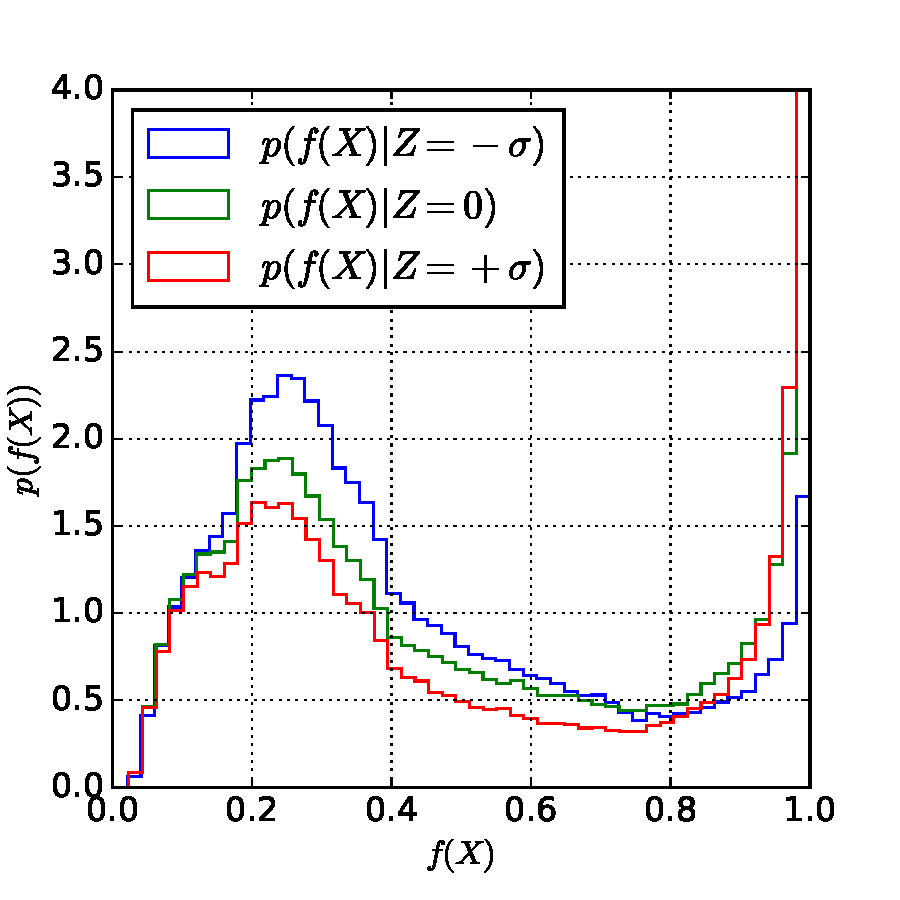
\includegraphics[width=0.245\textwidth]{figures/f-plain.pdf}
        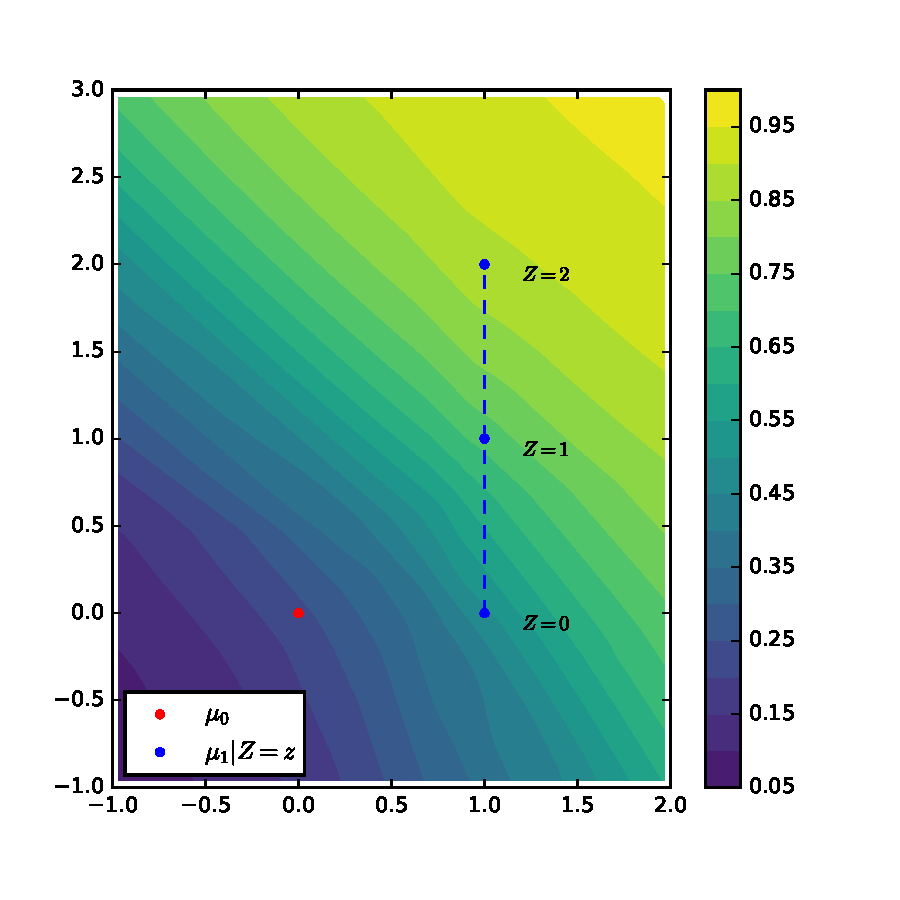
\includegraphics[width=0.245\textwidth]{figures/surface-plain.pdf}
        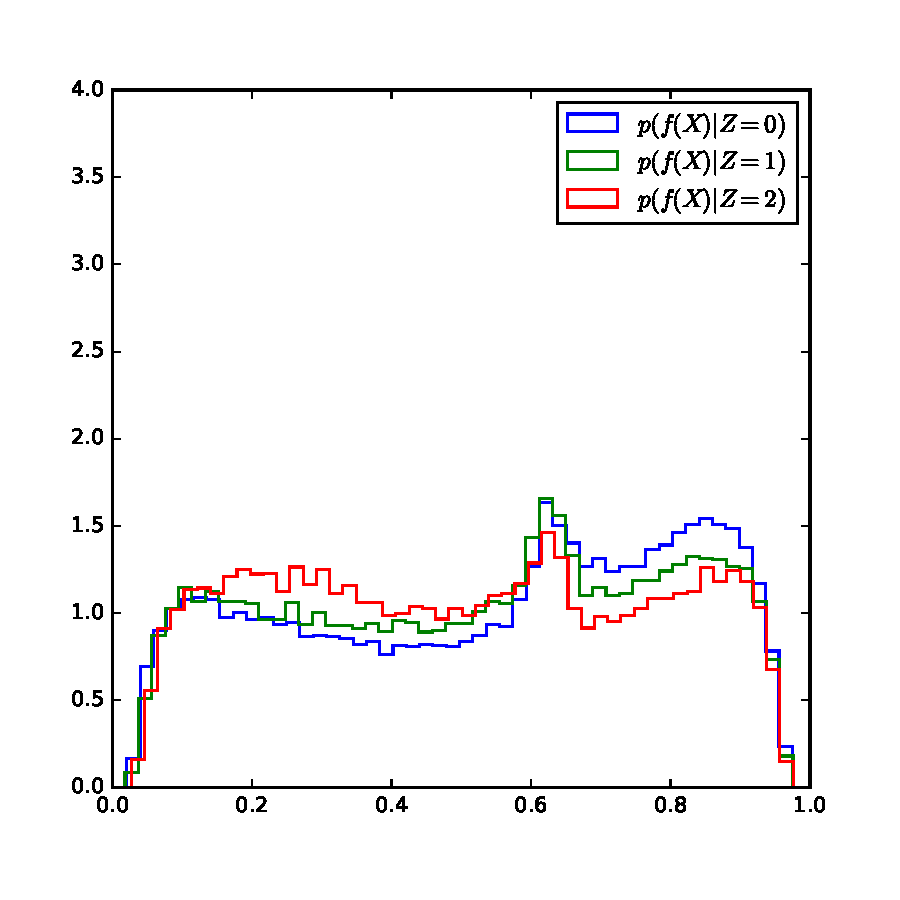
\includegraphics[width=0.245\textwidth]{figures/f-adversary.pdf}
        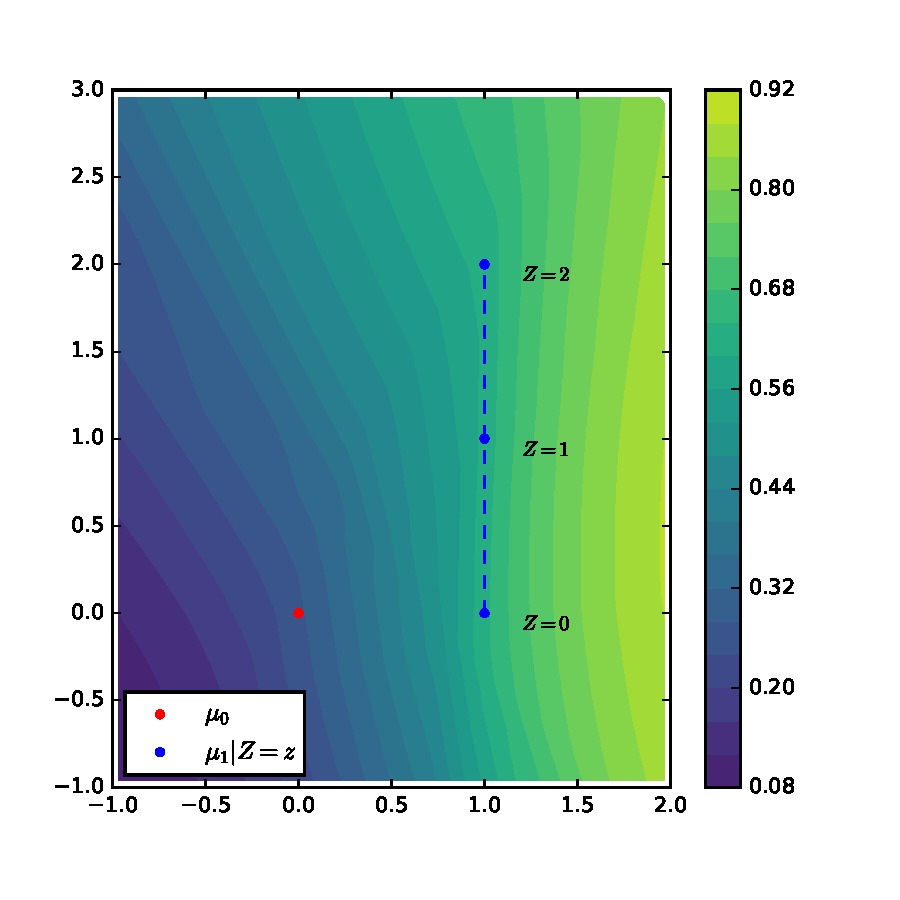
\includegraphics[width=0.245\textwidth]{figures/surface-adversary.pdf}
    \end{center}
    \vspace{-0.5cm}
    \caption{Toy example.
    (Left) Conditional probability densities of the decision scores at $Z=-\sigma, 0, \sigma$
       when $f$ is built without adversarial training. The resulting densities
       are clearly dependent on the continuous parameter $Z$, indicating that $f$ is not pivotal.
    (Middle left) The corresponding decision surface, highlighting
       the fact that samples are easier to classify for values of $Z$ above $\sigma$,
       hence partially explaining the dependency.
    (Middle right) Conditional probability densities of the decision scores at $Z=-\sigma, 0, \sigma$ when $f$ is
       built with adversarial training, as outlined in Sec.~\ref{sec:method}.
       The resulting densities are now almost identical to each other, indicating only a
       small dependency on $Z$.
    (Right) The corresponding decision surface, illustrating how adversarial
       training bends the decision function vertically to erase the dependency on $Z$.
    }
    \label{fig:toy}
\end{figure*}

\begin{figure}
    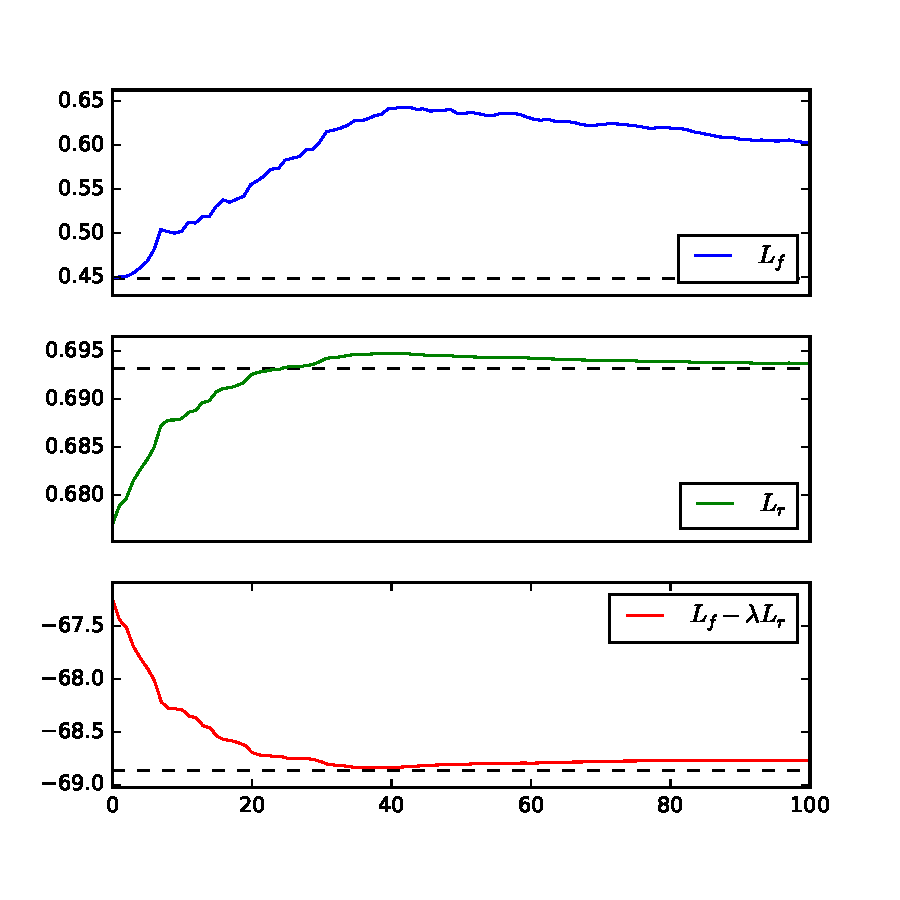
\includegraphics[width=0.48\textwidth]{figures/training.pdf}
    \vspace{-1cm}
    \caption{Toy example. Training curves for ${\cal L}_f(\theta_f)$, ${\cal L}_r(\theta_f, \theta_r)$
             and ${\cal L}_f(\theta_f) - \lambda {\cal L}_r(\theta_f, \theta_r)$.
             Adversarial training was performed for $200$ iterations, mini-batches of size $M=128$, $K=500$ and $\lambda=50$.}
    \label{fig:toy-training}
\end{figure}

As a guiding toy example, let us consider the binary classification of 2D
data drawn from multivariate gaussians with equal priors, such that
\begin{align}
    x &\sim {\cal N}\left ((0,0), \begin{bmatrix}
                              1 & -0.5 \\
                              -0.5 & 1
                            \end{bmatrix}\right) &\text{ when } Y=0, \\
    x &\sim {\cal N}\left ((1,1+Z),  \begin{bmatrix}
                              1 & 0 \\
                              0 & 1
                             \end{bmatrix}\right) &\text{ when } Y=1.
\end{align}
The continuous nuisance parameter $Z$ represents in this case our
uncertainty about the exact location of the mean of the second gaussian. Our goal is to
build a classifier $f(\cdot;\theta_f)$ for predicting $Y$ given $X$, but such that
the probability distribution of $f(X;\theta_f)$ is invariant with respect to the
nuisance parameter $Z$.

Assuming a gaussian prior $z \sim {\cal N}(0,1)$, we start by
generating training data $\{ x_i, y_i, z_i \}_{i=1}^N$, from which we train a
neural network classifier $f$ minimizing ${\cal L}_f(\theta_f)$ without
considering its adversary $r$. The network architecture comprises 2 dense hidden layers of 20
nodes with ReLU activations, followed  by a dense output layer with a single
node with a sigmoid activation. As shown in
Fig.~\ref{fig:toy}, the resulting classifier is not pivotal, as the
conditional probability densities of its decision scores $f(X;\theta_f)$ show
large discrepancies between values $z$ of the nuisance. While not shown here, a
classifier trained only from data generated at the nominal value $Z=0$ would
also not be pivotal.

Let us now consider the joint training of $f$ against an adversary $r$
implemented as a mixture density network modeling $Z|f(X;\theta_f)$ as a mixture
of five gaussians. As for $f$, the network architecture comprises 2 dense hidden
layers of 20 nodes with ReLU activations, but is followed by an output layer of
15 nodes corresponding to the means, standard deviations and mixture
coefficients of the five gaussians. Output nodes for the mean values come with
linear activations, output nodes for the standard deviations with exponential
activations to ensure positivity, while output nodes for the mixture coefficients
implement the softmax function to ensure positivity and normalization. When
running Algorithm~\ref{alg:adversarial-training} as initialized with the
classifier $f$ obtained previously, adversarial training effectively reshapes
the decision function so it that becomes almost independent on the nuisance
parameter, as shown in Fig.~\ref{fig:toy}. In particular,
the conditional probability densities of the decision scores $f(X;\theta_f)$ are
now very similar to each other, indicating only a small residual  dependency on the
nuisance, as theoretically expected. The dynamics of adversarial training is
illustrated in Fig.~\ref{fig:toy-training}, where the losses ${\cal L}_f$,
${\cal L}_r$ and ${\cal L}_f - \lambda {\cal L}_r$ are evaluated after each
iteration of Algorithm~\ref{alg:adversarial-training}. In the first iterations,
we observe that the global objective ${\cal L}_f - \lambda {\cal L}_r$ is
minimized by making the classifier less accurate, hence the corresponding
increase of ${\cal L}_f$, but which results in a classifier that is more
pivotal, hence the corresponding increase of ${\cal L}_r$ and the total net
benefit. As learning goes, minimizing $E$ then requires making predictions that
are more accurate, hence decreasing ${\cal L}_f$, or that are even less dependent on
$Z$, hence shaping $p_{\theta_r}$ towards the prior $p(z)$. Indeed, ${\cal L}_f$
eventually starts to  decrease, while remaining lower bounded by
$\min_{\theta_f} {\cal L}_f(\theta_f)$ as approximated by the dashed line in the
first plot. Similarly,  ${\cal L}_r$ tends towards the differential entropy
$H(Z)$ of the prior (where $H(Z) = \log(\sigma \sqrt{2 \pi e}) = 1.419$ in the
case of a gaussian with unit variance), as shown by the dashed line in the
second plot.
Finally, let us note that the ideal situation of a
classifier that is both optimal and pivotal appears to be unreachable for this
problem, as shown in the third plot by the  offset between ${\cal L}_f - \lambda
{\cal L}_r$ and the dashed line approximating $H({Y|X}) -
\lambda H(Z)$.

\subsection{High energy physics example}
\label{sec:hep}

%Experiments at high energy colliders like the LHC \citep{LHCMachine}
%are searching for evidence of new particles beyond the ones
%described by the so-called Standard Model (SM) of particle physics.
%A wide array of extended theories predict the existence of new massive
%particles that would decay to known heavy particles in the Standard Model,
%like the $W$, $Z$, Higgs boson, or top quark, which subsequently decay to
%multiple quarks.
%Finally, those quarks would produce collimated sprays of particles known as \textit{jets}.
%However, jets are produced ubiquitously at high energy colliders through
%more mundane processes in the SM, which leads to a challenging classification problem
%that is beset with a number of sources of systematic uncertainty.


Experiments at high energy colliders like the LHC \citep{LHCMachine}
are searching for evidence of new particles beyond the ones
described by the well established Standard Model (SM) of particle physics.
%Searches for these new particles in the LHC data involve a challenging
%classification problem that is beset with a number of sources of systematic uncertainty.
%
A wide array of extended theories predict the existence of new massive
particles that would decay to known particles in the SM such as the $W$ boson.
The $W$ boson is unstable and can decay to
two quarks, each of which produce collimated sprays of particles known as \textit{jets}
(collectively denoted $W\to jj$).
If the exotic particle is heavy, then the $W$ boson will be moving very fast,
and  relativistic effects will cause the two jets from its decay to merge into a single `fat jet'.
These fat jets have a rich internal substructure (see e.g.
\citep{Altheimer:2012mn,Altheimer:2013yza} and references therein).
However, jets are also produced ubiquitously at high energy colliders through
more mundane processes in the SM, which leads to a challenging classification problem
that is beset with a number of sources of systematic uncertainty.
%Distinguishing these ($y=1$) fat jets produced by heavy SM particles from
%the copious background of normal ($y=0$) jets is a fundamental challenge in searching
%for signs of new high mass particles.


%A wide array of extended theories predict the existence of new massive
%particles that would decay to known heavy particles in the Standard Model
%(e.g. the $W$ and $Z$ bosons), which subsequently decay to
%multiple quarks.
%Those quarks subsequently produce collimated sprays of particles known as \textit{jets} (denoted $j$).
%However, jets are produced ubiquitously at high energy colliders through
%more mundane processes in the SM, which leads to a challenging classification problem
%that is beset with a number of sources of systematic uncertainty.

%Consider the binary classification problem where $y=0$ corresponds to data produced from the
%ubiquitous SM process $pp \to jj$ and $y=1$ corresponds to data produced from an exotic
%process $pp \to W' \to W(\to jj) Z(\to jj)$ predicted by an extended theory.
%When the mass of the $W'$ is much larger than the mass of the $W$ and $Z$ bosons,
%then the $W$ and $Z$ particles are moving very fast and the relativistic Lorentz boost
%causes the two jets from their decay to merge into a single `fat jet',

%Consider the search for an exotic particle whose decay leads to a $W$ boson
%that subsequently decays to two jets via $W\to jj$.  If the $W$ boson is moving
%very fast, then the relativistic Lorentz boost
%causes the two jets from its decay to merge into a single `fat jet',
%which has a rich internal substructure (see e.g.
%\citep{Altheimer:2012mn,Altheimer:2013yza} and references therein).
%%We can cast this as a binary classification problem where $y=0$
%%corresponds to data produced from the ubiquitous SM process
%%that produce jets and $y=1$  corresponds to data produced from an exotic
%%process that gives rise to fat jets from $W\to jj$.


%binary classification problem where $y=0$ corresponds to data produced from the
%ubiquitous SM process $pp \to jj$ and $y=1$ corresponds to data produced from an exotic
%process $pp \to W' \to W(\to jj) Z(\to jj)$ predicted by an extended theory.
%When the mass of the $W'$ is much larger than the mass of the $W$ and $Z$ bosons,
%then the $W$ and $Z$ particles are moving very fast and the relativistic Lorentz boost
%causes the two jets from their decay to merge into a single `fat jet',
%which has a rich internal substructure (see e.g.
%\citep{Altheimer:2012mn,Altheimer:2013yza} and references therein).

%Distinguishing these ($y=1$) fat jets produced by heavy SM particles from
%the copious background of normal ($y=0$) jets is a fundamental challenge in searching
%for signs of new high mass particles.


The classification challenge used here is common in jet substructure
studies (see \citep{Khachatryan:2014vla,ATL-PHYS-PUB-2015-033,wbosonATLAS} and
references therein): we aim to discriminate between  the normal jets produced copiously
at the LHC ($Y=0$) and  the fat jets coming from an exotic process ($Y=1$).
We reuse the datasets used in
\citep{baldi2016jet}.  For completeness, the jets are built with the
anti-$k_T$ algorithm \citep{Cacciari:2008gp}
with radius parameter $R=1.2$, and trimmed \citep{Krohn:2009th} with subjets built with
the $k_T$ algorithm and parameter $f_{cut}=0.2$. The features used
in the classifiers are: trimmed jet invariant mass, N-subjettiness
$\tau_{21}^{\beta=1}$ \citep{nsub,Thaler2012}, and the energy correlation
functions  $C_{2}^{\beta=1}$, $C_{2}^{\beta=2}$,
$D_{2}^{\beta=1}$, $D_{2}^{\beta=2}$ \citep{Larkoski2013}.

Challenging in its own right, this classification
problem is made all the more difficult by the presence of pileup, or multiple
 proton-proton interactions occurring simultaneously with the primary
interaction.  These pileup interactions produce additional particles that can
contribute significant energies to jets unrelated to the underlying
discriminating information. The number of pileup interactions can vary with
the running conditions of the collider, and we want the classifier to be robust
to these conditions. Taking some liberty, we consider an extreme case with
a categorical nuisance parameter, where $Z=0$ corresponds to events without pileup
and $Z=1$ corresponds to events with pileup, for which there are an average  of
50 independent pileup interactions overlaid.

We do not expect that we will be able to find a function $f$ that simultaneously
minimizes the classification loss $L_f$ and is pivotal. Thus, we need to optimize
the hyper-parameter $\lambda$ of Eqn.~\ref{eqn:vf-lambda} with respect to
a higher-level objective. In this case, the natural higher-level context is a
hypothesis test of a null hypothesis with no $Y=1$ events against an
alternate hypothesis that is a mixture of $Y=0$ and $Y=1$ events.
In the absence of systematic uncertainties, optimizing $L_f$ simultaneously
optimizes the power of a classical hypothesis test in the Neyman-Pearson sense.
When we include systematic uncertainties we need to balance the
classification performance against the robustness to uncertainty in $Z$.
Since we are still performing a hypothesis test against the null, we only
wish to impose the pivotal property on $Y=0$ events. To this end,
we use the Approximate Median Significance (AMS), that was used
in the Higgs boson machine learning challenge that is a natural generalization
of the power of a hypothesis test when systematic uncertainties are taken into account
(see Eqn.~20 of \citep{adam2014higgs}).

%Our goal is to build an accurate classifier, for which we also want to minimize the effects due to the
%uncertainties on the nuisance. More specifically, we choose to recast the
%classification problem as a hypothesis test between signal+background (jets
%originating from $W$ bosons or from quarks and gluons) and background
%only (jets originating from quarks and gluons only) and tune the decision
%threshold of our classifier by maximizing its approximate median significance
%(AMS), when uncertainties in the background are taken into account (see Eqn.~20
%of \citep{adam2014higgs}). Our motivation is that reducing the effects of
%uncertainties by requiring independence of $Z$ with the classifier output $f(X;\theta_f)$ should
%allow for a larger maximum significance.

For several values of $\lambda$, we train a classifier
using  Algorithm~\ref{alg:adversarial-training} but consider the adversarial
term ${\cal L}_r$ conditioned on $Y=0$ only, as outlined in
Sec.~\ref{sec:problem}. Both $f$ and $r$ are neural networks with 3 hidden
layers of 64 nodes and ReLU activations, each terminated by a single final
output node with a sigmoid activation. Experiments are performed on a subset of
150000 samples for training while AMS is evaluated on an independent test set of
5000000 samples. Both training and testing samples are weighted such that the
null hypothesis corresponded to 10,000  of $Y=0$ events and the alternate
hypothesis included an additional 1,000 $Y=1$ events prior to any thresholding on $f$.
This allows us to probe the efficacy of the
method proposed here in a representative background-dominated high energy physics environment. 
Results reported below are averages over 5 runs.

\begin{figure}
    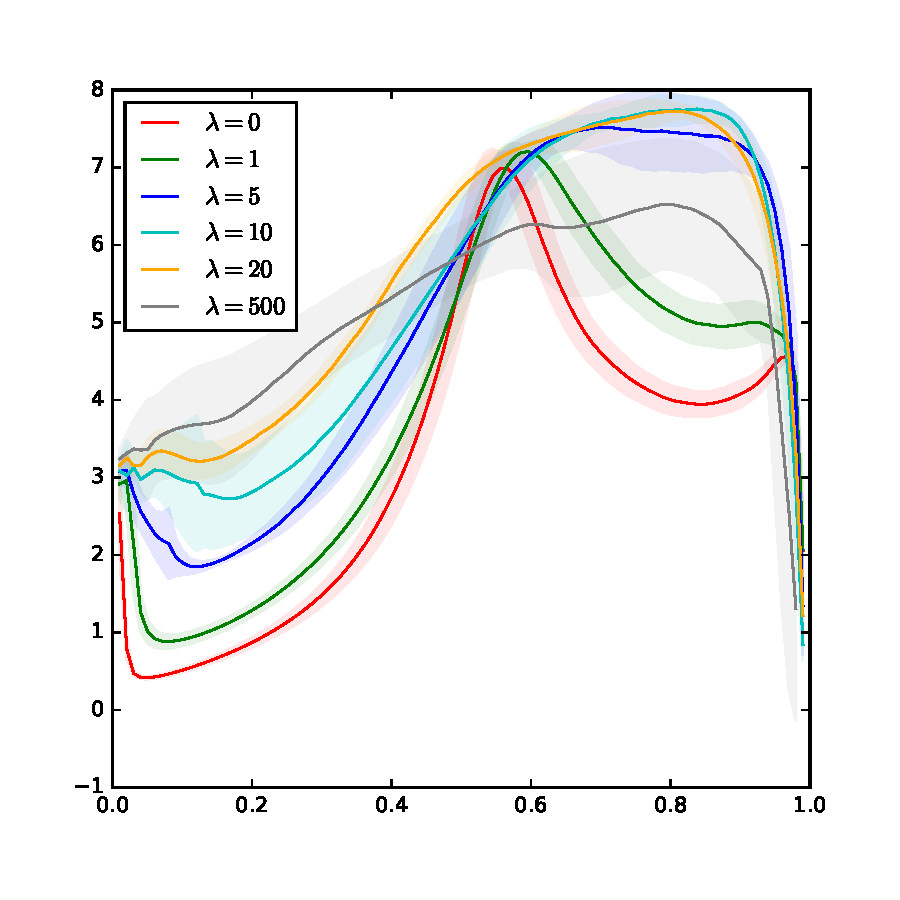
\includegraphics[width=0.48\textwidth]{figures/ams.pdf}
    \caption{Physics example. Approximate median significance as a function of the decision threshold
             on the output of $f$.  As shown at $\lambda=10$, trading
             classification accuracy for independence with respect to pileup
             results in a net benefit in terms of statistical significance.}
    \label{fig:physics-ams}
\end{figure}

As  Fig.~\ref{fig:physics-ams} illustrates, without adversarial training (at
$\lambda=0|Z=0$ when building a classifier at the nominal value $Z=0$ only, or
at $\lambda=0$ when building a classifier on data sampled from $p(X,Y,Z)$), the
AMS peaks at $7$. By contrast, as the pivotal constraint
is made stronger (for $\lambda > 0$) the AMS peak moves higher, with a maximum
value around  $7.8$ for $\lambda=10$. In other words, trading classification
accuracy for robustness to pileup results in a net
benefit in terms of the power of the resulting hypothesis test. Setting $\lambda$ too high however
(e.g. $\lambda=500$) results in a decrease of the maximum AMS, by
focusing the capacity of $f$ too strongly on independence with $Z$, at the expense of
classification accuracy. As demonstrated in this example, optimizing $\lambda$
gives us a principled and effective approach to control the trade-off between
accuracy and robustness that ultimately maximizes the
power of the enveloping hypothesis test.
%significance by desensitizing
%the classifier output $f(X;\theta_f)$ in the most beneficial way.


% ==============================================================================

\section{Related work}
\label{sec:related}

In machine learning, learning a pivotal quantity can be related to the problem
of domain adaptation
\citep{blitzer2006domain,pan2011domain,gopalan2011domain,gong2013connecting,baktashmotlagh2013unsupervised,ajakan2014domain,ganin2014unsupervised},
where the goal is often stated as trying to learn a domain-invariant
representation of the data. Likewise, our method also relates to the problem of
enforcing fairness in classification \citep{zemel2013learning,feldman2015certifying,EdwardsS15,zafar2015fairness}, which
is stated as learning a classifier that is independent of some chosen attribute
such as gender, color or age. For both families of methods, the problem can
equivalently be stated as learning a classifier which is a pivotal quantity with
respect to either the domain or the selected feature. In this context,
\citep{ganin2014unsupervised,EdwardsS15} are certainly among the closest to our
work, in which domain invariance and fairness are enforced through an
adversarial minimax setup composed of a classifier and an adversary
discriminator.
Following this line of work and without making assumptions on the prior $p(Z)$, our method can be regarded as a
generalization that also supports a continuously parametrized family of domains or as enforcing fairness over continuous attributes.
In that sense, our work is also original in the theoretical characterization
of the minimax solution of Eqn.~\ref{eqn:min_thetaf}.

To account for systematic uncertainties, experimentalists in high energy physics
typically take as fixed a classifier $f$ built from training data for a nominal
value $z_0$ of the nuisance parameter, and then propagate uncertainty
 by estimating $p(f(x)|z)$ with a parametrized calibration
procedure. Clearly, this classifier is however not optimal for $z \neq z_0$.
To overcome this issue, the classifier $f$ is sometimes built instead on a mixture
of training data generated from several plausible values $z_0, z_1, \dots$ of the nuisance parameter.
While this certainly improves classification performance with respect to the marginal model $p(X,Y)$,
there is no reason to expect the resulting classifier to be pivotal, as shown
previously in Sec.~\ref{sec:toy}.
As an alternative, parametrized
classifiers~\citep{cranmer2015approximating,Baldi:2016fzo} directly take
(nuisance) parameters as additional input variables, hence ultimately providing
the most statistically powerful approach for incorporating the effect of
systematics on the underlying classification task.  As argued in
\citep{Neal:2007zz}, it is not obvious how such classifiers can be used on real data since
the correct value $z$ of the nuisance often remains unknown. This is
not an issue in the context of parameter
inference~\citep{cranmer2015approximating}, where nuisance parameters are
eliminated via optimization or marginalization.
%, but otherwise often limits the range of their applications.
In practice, parametrized classifiers  are also computationally expensive to build
and evaluate. In particular, calibrating their decision function, i.e.
approximating $p(f(x,z)|y,z)$ as a continuous function of $z$, remains an open
challenge. By contrast, constraining $f$ to be pivotal yields a classifier which
may not be optimal with respect to $Y|X,Z$, as discussed in
Sec.~\ref{sec:theory}, but that can otherwise be directly used in a wider range of
applications, since the dependence on the nuisance parameter $Z$ has already been eliminated.
Moreover, if $f$ is sufficiently close to being pivotal, then calibration only needs to be carried out once.


%Following this line of work and without making assumptions on the prior $p(Z)$, our method can be regarded as a
%generalization that also supports the continuous case, which can be viewed as
%handling infinitely many domains, provided they can be continuously
%parametrized, or as enforcing fairness over continuous attributes.


% ==============================================================================

\section{Conclusions}
\label{sec:conclusions}

In this work, we proposed a flexible learning procedure for building a
predictive model that is independent of continuous or categorical nuisance
parameters by jointly training two neural networks in an adversarial fashion.
From a theoretical perspective, we motivated the proposed algorithm by showing
that the minimax value  of its value function corresponds to a predictive model
that is both optimal and pivotal (if that models exists) or for which one can
tune the trade-off between power and robustness. From an empirical point of
view, we confirmed the effectiveness of our method on a toy example and particle physics example.

Despite the theoretical characterization of the minimax solution of Eqn.~\ref{eqn:min_thetaf}
that motivates this work,
Algorithm~\ref{alg:adversarial-training} remains a heuristic in the sense
that we do not provide formal guarantees of convergence of the procedure towards
that solution. Empirical evidence gathered here and in similar minimax-based
related works (see e.g., \citep{goodfellow2014generative,EdwardsS15}) suggests
that the alternating optimization algorithm works sufficiently well in practice,
but further research studying its stability and convergence would certainly
be beneficial for a large body of works.

In terms of applications, the proposed solution can be used in any situation
where the training data may not be representative of the real data the
predictive model will be applied to in practice. In the scientific context, this
includes situations where the data generation processes are associated to
systematic uncertainties (e.g., as in high energy physics), and which would be
worth revisiting in light of the proposed solution. More generally, the approach
also extends to cases where independence of the predictive model with respect to
random variables is desired, as in domain adaptation or fairness in
classification. Again, trying our algorithm on these use cases is certainly
worth investigating.

\bigskip

% ==============================================================================

\begin{acknowledgments}

    We would like to thank the authors of Ref.\citep{baldi2016jet} for sharing the data used in their
    studies.
    KC and GL are both supported through NSF ACI-1450310, additionally KC is supported
    through PHY-1505463 and PHY-1205376. 

\end{acknowledgments}


\vfill

% ==============================================================================

\bibliographystyle{acm}
\bibliography{bibliography.bib}

\vfill

\end{document}
